\documentclass[10pt]{article}
% --- BASIC PACKAGES ---
\usepackage[utf8]{inputenc}
\usepackage{amsmath, amssymb, amsfonts} % For advanced math
\usepackage{graphicx}                   % For including images
\usepackage[a4paper, margin=1in]{geometry} % Set page margins
\usepackage{hyperref}                   % For clickable links and citations
\hypersetup{
    colorlinks=true,
    linkcolor=blue,
    filecolor=magenta,      
    urlcolor=cyan,
    citecolor=red,
}
% --- CHINESE LANGUAGE SUPPORT ---
\usepackage{ctex} % Kept from your original for Chinese characters
% --- BIBLIOGRAPHY (using biblatex) ---
% Switched to biblatex for modern citation management. It works well with \citet.
% You will need to compile with: pdflatex -> biber -> pdflatex -> pdflatex
\usepackage[backend=biber,style=gb7714-2015ay]{biblatex}
%biblatex宏包的参考文献数据源加载方式
\DefineBibliographyStrings{english}{
  andincite = {和},
  andincitecn = {和},
  andothersincite = {等},%adddot才能避开标点追踪
  andothersincitecn = {等}, }
\addbibresource{ref.bib} % Assumes your bibliography file is ref.bib
% --- CUSTOM COMMANDS ---
\newcommand{\his}{\textsuperscript{\ddag}}
% --- DOCUMENT METADATA ---
\title{湍流唯象学 \\ \large 吉奥亚\his 的方法}
\author{刘宁 \\ \textit{浙江大学}} % Institute is often placed under the author
\date{\today}
\begin{document}
\maketitle
\begin{abstract}
本文概述了基于吉奥亚(Gioia)及其合作者所发展的方法对湍流现象学的描述。我们回顾了速度尺度的表达形式、局部剪切应力模型及其在不同流动区域的统一,并与其他经典模型进行了比较。
\end{abstract}

\section{尺度 $s$ 上的速度分量}
尺度为 $s$ 的速度分量的平方可通过能量谱的积分来表示,该积分可对空间尺度 $\sigma$ 或波数 $k$ 进行:
\begin{align*}
    u_s^2 = \int_0^s E(\sigma) \sigma^{-2} d\sigma = \int_{1 / s}^{\infty} E(k) dk
.\end{align*}
能量谱 $E$ 受耗散区($\mathbf{c_d}$)和含能区($\mathbf{c_e}$)的修正函数调制:\footnote{注:\citet{gioiaFriction2006} 使用的形式为 $\mathbf{c_e} \left( \sigma / R \right)$。我们注意到 $R / \sigma = Rk$,因此为了使 $\mathbf{c_e}$ 的表达形式统一,我们将其定义为 $\mathbf{c_e} \left( R / \sigma \right)$。}
\begin{align*}
    E(\sigma) &\sim \varepsilon^{2 / 3} \sigma^{5 / 3} \mathbf{c_d} \left( \frac{\eta}{\sigma} \right) \mathbf{c_e} \left( \frac{R}{\sigma} \right) \\
    E(k) &\sim \varepsilon^{2 / 3} k^{-5 / 3} \mathbf{c_d} (\eta k) \mathbf{c_e} \left( \frac{1}{Rk} \right).
\end{align*}
修正函数的具体形式为:
\begin{align*}
    \begin{cases}
        \mathbf{c_d}\left( x \right)  = \exp\left( -\beta_d x \right) \\
        \mathbf{c_e} \left( x \right) = \left( 1+\beta_e x^{-2} \right) ^{-17 / 6} 
    \end{cases}
.\end{align*}
其中 $\mathbf{c_d}$ 的形式来自 \citet{gioiaFriction2006},而 $\mathbf{c_e}$ 则取自冯·卡门(von Kármán)。在惯性区($\eta \ll s \ll R$),两个修正项均趋近于 1。\footnote{为何调整耗散区和含能区的系数无法导出常见的 $-1$ 标度律?参见 \cite{nikora1999prl},假设当涡体尺度由外区标度控制($1 / H \ll k \ll 1 / z$)时,引入 $\varepsilon(k) \sim u_{\tau }^3 k$。}

\section{速度 $u_s$ 的统一表达形式}
令 $\xi = sk = s / \sigma$,可将 $u_s$ 写成统一形式:
\begin{align*}
    u_s \sim \left( \varepsilon s \right) ^{1 / 3} \left[ \int_1^{\infty} \xi^{-5 / 3} \mathbf{c_d}\left( \frac{\eta}{s} \xi \right) \mathbf{c_e} \left( \frac{R}{s} \xi \right) d\xi \right]^{1 / 2}  \triangleq \left( \varepsilon s \right) ^{1 / 3} \sqrt{\mathcal{I} } 
.\end{align*}
\paragraph{核心要点。}

    
- 在惯性区($\eta \ll s \ll R$),速度满足标度关系 $u_s \sim \left( \varepsilon s \right) ^{1 / 3} $。
    
- 确定尺度为 $s$ 的涡体的特征速度 $u_s$ 的问题,转化为对修正函数 $\mathcal{I}\left( \eta / s, R / s \right)$ 的分析,其定义为:
    \[
        \mathcal{I}\left( \frac{\eta}{s}, \frac{R}{s} \right)  \triangleq \int_1^{\infty} \xi^{-5 / 3} \mathbf{c_d}\left( \frac{\eta}{s} \xi \right) \mathbf{c_e} \left( \frac{R}{s} \xi \right) d\xi.
    \]


\section{现象学的整体图景}
该模型建立在能量级串(energy cascade)的概念之上。

    
- \textbf{能量级串}:能量在不同尺度间的传递速率是恒定的。
        \begin{align*}
            u_s^3 / s \sim u_R^3 / R
        .\end{align*}
        
            
- 由 $\varepsilon \sim u_R^3 / R$,可得柯尔莫哥洛夫尺度 $\eta = \left( 
u^3 / \varepsilon \right)^{1 / 4}\sim R\cdot Re^{-\frac{3}{4}} $。
            
- 由 $\varepsilon  \sim {u_{\tau }^3}/{\kappa y}$ 和 $u_s\sim \left( \varepsilon s \right) ^{1 / 3} $,对于惯性区涡体(特别是在对数层中,$s \sim y$)\footnote{因此,在外层(忽略粘性底层),负责动量混合的涡体其特征速度自然为 $u_{\tau }$。}:
                $$u_s \sim u_{\tau } \left( s / y \right) ^{1 / 3} \sim u_{\tau}.$$ 
            
- \textbf{关于 $C_f$ 标度的不一致(?)}:\citet{gioiaFriction2006} 将摩擦系数表示为 $C_f \sim u_s / V \sim u_{\tau } / V$。然而,根据摩擦速度和摩擦系数的定义,应有 $C_f \sim \tau / V^2 \sim u_{\tau }^2 / V^2$。
        


\section{吉奥亚的方法:局部剪切应力模型}
跨越湿表面 $W_y$ 的尺度为 $(u_s, s)$ 的涡体会产生剪切应力 $\tau$。该模型将其概念化为动量传递速率($v_n$)与所传递动量大小($v_t$)的乘积。

    
- $v_n$ 表示涡体传递动量的速率,取决于其特征速度($\sim u_s$)。
    
- $v_t$ 表示涡体可传递的动量大小,取决于湿表面积上的动量差($\propto \frac{\partial u}{\partial y}\cdot s $)。

剪切应力建模为:
\begin{align*}
    \tau \sim \rho v_t v_n
.\end{align*}
\begin{figure}[ht!]
    \centering
    \includegraphics[width=0.4\textwidth]{./figures/eddies.png}
    % \caption{Schematic of eddy phenomenology \cite{gioiaprl2001}.}
    \label{fig:-figures-eddies-png}
\end{figure}
该模型根据位置不同而有所应用:

    
- \textbf{局部壁面剪切应力模型} \cite{gioiaFriction2006}:$v_t \sim V$,$v_n\sim u_{k_s+a\eta}$。
    
- \textbf{局部水柱剪切应力模型} \cite{gioiaMVP2010}:$v_t\sim u(y+s) - u(y-s)\approx 2s u'(y) \sim 2y\cdot u'(y)$,$v_n \sim u_y$。

\begin{figure}[!htb]
    \centering
    \begin{minipage}{.5\textwidth}
        \centering
        \includegraphics[width=0.7\textwidth]{./figures/wall-shear.png}
        \caption{壁面剪切应力模型。}
        \label{fig:wall-shear}
    \end{minipage}%
    \begin{minipage}{0.5\textwidth}
        \centering
        \includegraphics[width=0.7\textwidth]{./figures/column-shear.png}
        \caption{水柱剪切应力模型。}
        \label{fig:column-shear}
    \end{minipage}
\end{figure}

\section{局部剪切应力模型的统一}
\subsection{统一图景}
\begin{figure}[htpb]
    \centering
    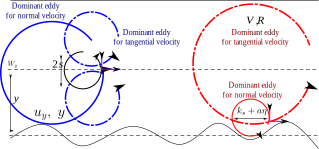
\includegraphics[width=0.8\textwidth]{./figures/unify-gioia-model.pdf}
    \caption{吉奥亚模型的统一图景。}
    \label{fig:-figures-unify-gioia-model-pdf}
\end{figure}
其核心思想是根据涡体的位置和尺度来定义动量的“运输者”($v_n$)和“货物”($v_t$)。

    
- \textbf{运输者($v_n$)}:靠近床面时,特征涡体尺度受粗糙度高度 $k_s$ 和粘性底层厚度 $a\eta$ 共同控制,因此 $s = k_s + a\eta$\ddag。在外区,特征涡体尺度由离壁距离决定,即 $s\sim y$。\footnote{汤森德(Townsend)的附着涡假设提出了一系列自相似涡体,其特征尺度与壁面距离成正比。这可视为仅考虑外层涡体的特例,因此附着涡模型主要适用于对数律区 \cite{aemmarusic2019}。}
    
- \textbf{货物($v_t$)\his}:负责 $v_n$ 分量的涡体充当动量运输者。其空间尺度决定了它能携带的动量 $v_t$ 的大小。\footnote{因为对于给定的涡体空间尺度 $s$,在此距离上覆盖的速度梯度是 $s$ 的函数。}
        
            
- 一旦涡体尺度 $s$ 确定,$v_n$ 和 $v_t$ 是否同时确定?如果是这样,大涡叠加在小涡上的模型可能不再必要。我们只需引入“运输者”涡体,类似于附着涡模型。
            
- 外区由于速度梯度可传输的动量差为:
            $$v_t \sim 2s u'(y) \sim 2y \cdot u'(y).$$
            
- 壁面附近的动量差\his 为\footnote{这导致了过渡粗糙区的斯特里克勒(Strickler)型关系:$\tau_0 \propto \left( k_s / R \right) ^{\frac{1}{3}} \rho V^2 $。}:
            $$\lim_{y \to 0} v_t \sim \left( k_s + a\eta \right) \lim_{y \to 0} u'(y) =  \frac{(k_s + a \eta)u_{\tau}^2}{
u} \sim (k_s + a\eta) \frac{\left( k_s / R \right)^{\frac{1}{3}} V^2}{
u}.$$
            上述式子显然不单单与平均流速 $V$ 成比例,而是与雷诺数 $Re = \left( k_s + a\eta \right) V / 
u$ 相关。因此在考虑内标度范围的近壁区域,涡体所能交换的动量差无法直接以 \citet{gioiaprl2001} 中大小涡体叠加模型的 $V$ 作为特征速度。
        


\subsection{涡体作为动量扩散系统}
尺度为 $(V, R)$ 的涡体可被视为一个动量扩散系统 $\mathcal{D}_e \propto VR$ \cite{ocfjfm2024}。\footnote{此时我们已超越流场中具体流体运动的可视化,不再试图从流场中捕捉抽象的涡体。这种视角与普朗特(Prandtl)的混合长度理论类似。} 这种视角突显了一个基本对比:

    
- 层流通量由分子扩散驱动($\propto 
u$)。
    
- 湍流通量由最大尺度涡体和回流单元的扩散驱动($\propto VR$)。
    
- 雷诺数 $Re = \frac{VR}{
u}$ 代表了湍流与层流驱动机制的比值。

由涡体 $(V, R)$ 产生的动量通量 $F$ 可表示为\footnote{论文中第二种情况的推导可能存在循环论证的风险。} \cite{ocfjfm2024}:
\begin{align*}
    F \sim \rho \left[ (VR)^2 \right] '\sim -\rho \int_0^{R}  \mathcal{D}_e \frac{\partial u}{\partial y} dz
.\end{align*}
\begin{figure}[ht!]
    \centering
    \includegraphics[width=0.6\textwidth]{./figures/momentum-flux.png}
    \caption{通道部分区域的动量平衡,来自 \cite{ocfjfm2024}。}
    \label{fig:-figures-momentum-flux-png}
\end{figure}

\section{吉奥亚涡体模型 vs. 附着涡体模型}
\textit{(内容待补充。)}

\section{吉奥亚涡体模型 vs. 涡粘性模型}
\textit{(内容待补充。)}

\section{吉奥亚涡体模型在时均场视角下的表现}
\textit{(内容待补充。)}

\section{吉奥亚涡体模型与 LSM/VLSM}
\subsection{“-1” 标度律在湍流现象学视角下的解释}
\citet{nikora1999prl} 借助涡体能量级串的唯象学进行解释:特定尺度 $\frac{1}{k}$ 的涡体能量通量等于所有更大尺度涡体能量通量与其自身动量通量的叠加,直至达到惯性区尺度的涡体(外标度不再起作用,局部各向同性,OK41 理论),此时动量通量为常值 $\varepsilon_d$。
\begin{figure}[htpb]
    \centering
    \includegraphics[width=0.8\textwidth]{./figures/energy-cascade.png}
    \caption{在 $z_3$ 处测量、由所有可能的 $z$ 处发起的能量级串叠加效应 \cite{nikora1999prl}。}
    \label{fig:-figures-energy-cascade-png}
\end{figure}
将外区涡体的能量通量 $\varepsilon(k)$
\begin{figure}[htpb]
    \centering
    \includegraphics[width=0.6\textwidth]{./figures/cascade.pdf}
    \caption{外区能量通量级串。}
    \label{fig:-figures-cascade-pdf}
\end{figure}

\section{未来展望}

    
- 局部剪切应力模型 $\implies$ 一种新的亚格子应力模型。
    
- 一种新的亚格子应力模型 $\implies$ 网格优化器。


% --- BIBLIOGRAPHY ---
\printbibliography[heading=bibintoc, title={参考文献}]
\end{document}
